% VLDB template version of 2020-08-03 enhances the ACM template, version 1.7.0:
% https://www.acm.org/publications/proceedings-template
% The ACM Latex guide provides further information about the ACM template

\documentclass[sigconf, nonacm]{acmart}

%% The following content must be adapted for the final version
% paper-specific
\newcommand\vldbdoi{XX.XX/XXX.XX}
\newcommand\vldbpages{XXX-XXX}
% issue-specific
\newcommand\vldbvolume{14}
\newcommand\vldbissue{1}
\newcommand\vldbyear{2020}
% should be fine as it is
\newcommand\vldbauthors{\authors}
\newcommand\vldbtitle{\shorttitle} 
% leave empty if no availability url should be set
\newcommand\vldbavailabilityurl{https://doi.org/10.5281/zenodo.10706620}
% whether page numbers should be shown or not, use 'plain' for review versions, 'empty' for camera ready
\newcommand\vldbpagestyle{plain} 

\begin{document}
\title{RepEng Project: An Approach for Schema Extraction of JSON and Extended JSON Document Collections}

%%
%% The "author" command and its associated commands are used to define the authors and their affiliations.
\author{Kachimsirikwuo Caleb Imo}
\affiliation{%
  \institution{Universität Passau}
  \streetaddress{P.O. Box 1212}
  \city{Passau}
  \state{Germany}
}
\email{imo01@ads.uni-passau.de}


\maketitle

%%% do not modify the following VLDB block %%
%%% VLDB block start %%%
\ifdefempty{\vldbavailabilityurl}{}{
\vspace{.3cm}
\begingroup\small\noindent\raggedright\textbf{Artifact Availability:}\\
The source code, data, and/or other artifacts have been made available at \url{\vldbavailabilityurl}.
\endgroup
}
%%% VLDB block end %%%
\section{Introduction}
This project report aims to reproduce the findings presented in the original paper \cite{frozza2018approach}. The original study introduced an innovative approach to extracting JSON or Extended JSON schema from large datasets.

The introduction of NoSQL databases has revolutionized data storage by enabling the storage of diverse data collections without requiring a predefined structure. However, the absence of an explicitly stated schema does not imply the absence of an implicit schema \cite{sevilla2015inferring, frozza2018approach}
. The proposed approach in \cite{frozza2018approach}, termed JSON Schema Discovery, aims to extract a unified schema from a collection of JSON documents, catering to applications that may necessitate such schema information.

\section{TOOL EVALUATION}\label{sec:tool_eval}
To evaluate the quality of the JSON Schema Discovery approach, three experiments were conducted using diverse collections of JSON documents stored in a MongoDB. 
Table~\ref{dbpedia} shows a comparative analysis of schema extraction between JSON Schema Discovery and the method described by Wang et al. \cite{wang2015schema}, using datasets retrieved from DBPedia. The following terms are derived from the column labels used in Table~\ref{dbpedia}:

\begin{table}
\centering
\caption{Original table of JSON schema extraction from \cite{frozza2018approach}}\label{dbpedia}
\scalebox{0.80} {
\begin{tabular}{|l|c|c|c|c|}
\hline
\multicolumn{2}{|c|}{\textbf{Datasets}} & \multicolumn{2}{c|}{\textbf{JSON Schema Discovery}} & \textbf{Wang et al.} \cite{wang2015schema}\\
\hline
\textbf{Collection} & \textbf{N\_JSON} & \textbf{RS} & \textbf{ROrd} & \textbf{FS} \\
\hline
drugs & 3662 & 2818 & 2818 & 2818 \\
\hline 
companies & 24367 & 21312 & 21312 & 21302 \\
\hline
movies & 30330 & 25140 & 25140 & 25137 \\
\hline
\end{tabular}
}
\end{table}

\begin{description}
  \item[\textbullet] \textbf{N\_JSON}: Number of JSON documents.
  \item[\textbullet] \textbf{RS}: Number of raw schemas generated.
  \item[\textbullet]\textbf{ROrd}: Number of distinct raw schemas generated with an ordered structure.
  \item[\textbullet]\textbf{FS}: Number of final schemas generated by the approach described in Wang et al. \cite{wang2015schema}.
\end{description}

The first column in Table~\ref{dbpedia} shows the three categories along with the total number of JSON documents that were used as datasets for this experiment. The second column indicates the results of both unordered and ordered schemata generated by the JSON Schema Discovery tool. The third column represents the number of final schemas generated using the approach proposed by Wang et al. \cite{wang2015schema} on the same dataset. This means that the JSON documents categorized as datasets containing details about companies, totaling 3662 records, produced a consistent total of 21312 schemas when generated by the JSON Schema Discovery tool, regardless of whether they were ordered or unordered. In contrast, the approach proposed by Wang et al. \cite{wang2015schema} yielded 21302 schemas for the same dataset.

\subsection{Research Question}\label{subsec:research}
\textbf{RQ:} Given identical datasets, does the execution of the experiment using the methodology outlined in the original research paper reproduce similar outcomes?

The research question aims to verify the consistency and accuracy of the reported findings, as outlined in Table~\ref{dbpedia}. It is important to emphasize that this study focuses solely on reproducing the results obtained from the JSON Schema Discovery tool and will not endeavor to reproduce the findings labeled '\textit{FS}' in Table~\ref{dbpedia}, as documented by Wang et al. \cite{wang2015schema}.

To validate the results of this reproduction report, a comprehensive comparison will be conducted between the output values of the generated schemas and those reported in the original paper.
 
Before executing the reproduction experiment, a manually crafted CSV file documenting the results of the JSON Schema Discovery tool as described by Frozza et al. \cite{frozza2018approach} will be prepared. This file will serve as a reference for comparison against the CSV file generated from the experiment. A hash comparison will be conducted on the files to ensure an exact match between the generated and the manually crafted results present in the reproduction repository.  In a situation where they differ, a differential analysis will then be performed to identify any differences between the two sets of results. This step will help confirm the accuracy and consistency of the reproduced findings. 

This reproduction report is primarily concentrated on validating the experimental results presented in Table \ref{dbpedia}. As a result, it will not attempt to reproduce every other experiment mentioned in \cite{frozza2018approach}. This focused scope ensures a thorough examination of specific findings outlined in the original paper.

\section{Reproduction Package}
In this section, we thoroughly examine the setup environment for our reproduction experiment, present the obtained results, and compare them with those documented in the original paper.

\subsection{Setup Environment}
To facilitate the execution of the JSON Schema Discovery tool,  a containerized environment was established using Docker for streamlined rebuilding. Additionally, patches were implemented to address broken code resulting from dependency failures, as certain dependencies were deemed obsolete at the time of reproduction.

The core codes of the original tool remain unaltered, distinguishing this effort as a reproduction rather than a replication. Only adjustments to dependencies and the version of MongoDB for storing JSON documents were made, preserving the original tool's structure. The datasets used in the original study were utilized for this reproduction experiment. These datasets are automatically pulled into the container environment during the build process. By utilizing a containerized environment, all necessary dependencies for running the JSON Schema Discovery tool are made available upon container startup, thereby simplifying the reproduction process for other interested readers.

The experiment in the original research paper, as depicted in Table~\ref{dbpedia}, were conducted on an ASUS K45VM notebook (Intel® Core ™ i7 3610QM @ 2.30 GHz and 8GB of RAM)\cite{frozza2018approach}. In contrast, the reproduction of this experiment was conducted on an ACER Aspire A515-55 system ( Intel(R) Core(TM) i5-1035G1 CPU @ 1.00GHz). However, given that the focus is not the execution time of the tool, we can assert that the difference between the two systems does not impact the results in terms of the total number of schemas generated, whether ordered or not.

\begin{table}
\centering
\caption{Comparison of Generated Schema Values from Reproduction Script Execution} \label{reprod_latex}
\scalebox{0.80} {
\begin{tabular}{|l|c|c|c|c|c|}
\hline
\multicolumn{2}{|c|}{\textbf{Datasets}} & \multicolumn{2}{c|}{\textbf{JSON Schema Discovery}} &
\multicolumn{2}{c|}{\textbf{Frozza et al. \cite{frozza2018approach}}} \\
\hline
\textbf{Collection} & \textbf{N\_JSON} & \textbf{RS} & \textbf{ROrd} & \textbf{RS} & \textbf{ROrd} \\
\hline
%ROWS%

\end{tabular}
}
\end{table}

\subsection{Execution and Result}
Table~\ref{reprod_latex} displays the results of executing the reproduction script alongside the findings of Frozza et al. \cite{frozza2018approach}. The column labels remain consistent with the descriptions outlined in Section~\ref{sec:tool_eval} of this report. 
The first column lists the datasets used in this reproduction experiment. The second column indicates the number of generated schemas, including both raw and ordered structured schemas, produced from the reproduction environment. The third column displays the number of schemas, both raw and ordered structured generated schemas, as documented by Frozza et al.~\cite{frozza2018approach}.

According to Table~\ref{reprod_latex}, which utilized the same datasets as documented in the original paper, it is apparent that the reproduction process yielded a consistent number of schemas across all categories, including raw and ordered structure schemas.

To confirm the reproducibility of this experiment, a CSV file was generated after executing the tool to document the total number of schemas for each category, utilizing Python's csv module. Following this, the resulting CSV file was compared with the manually created CSV file, as discussed in subsection~\ref{subsec:research}.

The rationale behind the comparison process was to use a hash-based checksum to analyze the hashes of both CSV files. When the hashes match, it confirms the success of the experiment. However, if the hashes differ, a differential analysis is triggered to identify any discrepancies between the files. If no differences are found, it indicates that both CSV files contain identical content,  thereby validating the success of the experiment despite the hash mismatch. Conversely, if differences are detected, it implies a failure of the reproduction experiment.

 \begin{figure}
     \centering
     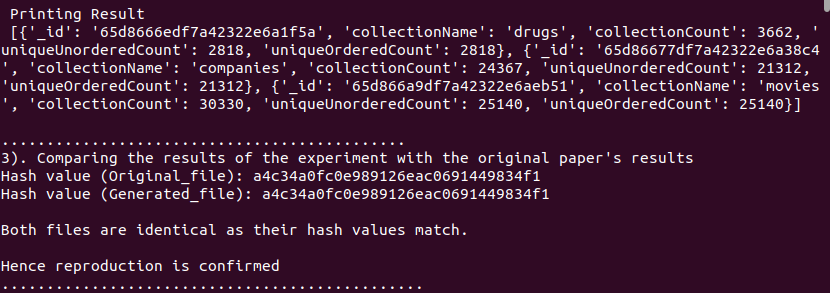
\includegraphics[height=0.2\textwidth, width=0.5\textwidth]{img/experiment.png}
     \caption{comparison of both csv files }
     \label{fig:experiment}
 \end{figure}

At the time of conducting this reproduction experiment, the comparison indicated that both CSV files were identical, as shown in Figure~\ref{fig:experiment}. This confirmation validates that the reproduction of the experiment conducted by Frozza et al. \cite{frozza2018approach} was indeed successful.

\subsection{Limitations to Validity}
The validation of the reproduced results posed somewhat a challenge due to the unavailability of the original paper's results in a compatible format for direct comparison. The results presented by Frozza et al. \cite{frozza2018approach} were only available in a tabular format within their report and were not accompanied by any accessible JSON or CSV files. To address this challenge, a manually crafted CSV file was generated prior to the execution, thereby providing a reference point for comparison. This crafted CSV file was meticulously created by referencing Table~\ref{dbpedia} from the original paper.

\subsection{Conclusion}
The aim of this report was to reproduce the experiment conducted by Frozza et al. \cite{frozza2018approach}, as outlined in Table~\ref{dbpedia}. To achieve this, a containerized environment was established, incorporating necessary patches to ensure the successful execution of the experiment. The reproduction process yielded results consistent with those documented in the original research paper, thereby confirming the success of the reproduction experiment.



\bibliographystyle{ACM-Reference-Format}
\bibliography{sample}

\end{document}
\endinput
